	Rozdział poświęcony jest ogólnemu opisowi działania poszczególnych fragmentów aplikacji zarówno od strony jej użytkownika jak i kodu źródłowego.

\section{Interfejs użytkownika}
	Graficznym interfejsem użytkownika (GUI) jest prosty formularz HTML, domyślnie dostępny w oknie przeglądarki internetowej po uruchomieniu aplikacji pod adresem lokalnego hosta na porcie 8080: 
	\smallbreak
	\href{http://localhost:8080/flowchart/}{localhost:8080/flowchart/}.
	\bigbreak	
	Domyślnie GUI zawiera w górnej części pole z wygenerowanym diagramem blokowym, a pod nim  menu rozwijane umożliwiające wybór składni kodu zarówno Mermaid jak i C-podobnego (dropdown select menu), pole tekstowe (text area) do wprowadzania samego kodu oraz przycisk potwierdzający przesłanie typu wybranej składni i kodu przez Rest API. Żądanie typu GET obsługiwane przez kontroler Rest dopuszczający dwa opcjonalne parametry: typ składni ($type$) - domyślnie przyjmujący składnie Mermaid, kod umieszczony w polu tekstowym ($originalCode$) - domyślnie rysujący dwa proste bloczki. Jakiekolwiek wyrzucenie wyjątku przez program zostaje obsłużone właśnie w kontrolerze, po czym przekazana zostaje wiadomość w nim zawarta do ekranu błędu.

	
\begin{figure}[H]
  \begin{subfigure}{\textwidth}
    \centering
    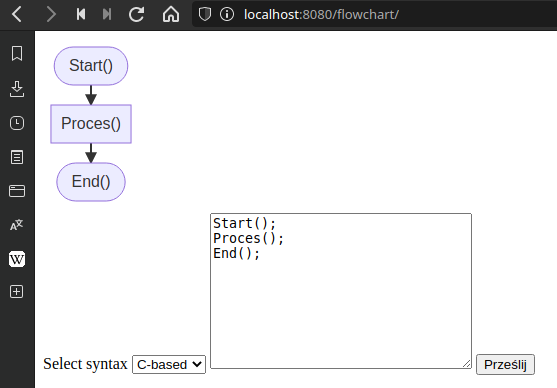
\includegraphics[width=0.8\textwidth]{GUI.png}
  \end{subfigure}\hfill
  \caption{Interfejs graficzny użytkownika wyświetlony przy pomocy przeglądarki Vivaldi 5. }
\end{figure}

Przykładowy schemat blokowy dostępny pod adresem: 
	\smallbreak
	\href{http://localhost:8080/flowchart/?type=C\&originalCode=Start();Proces();End();}{http://localhost:8080/flowchart/?type=C\&originalCode=Start();Proces();End();}
	\bigbreak
	
	Dodatkowym ekranem jest strona HTML, która wyświetla komunikat o błędzie składniowym oraz pokazuje fragment kodu w którym ten błąd nastąpił.
	
\begin{figure}[H]
  \begin{subfigure}{\textwidth}
  \centering
    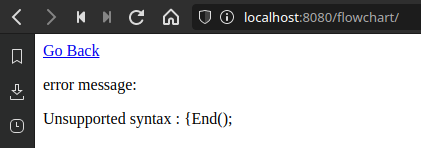
\includegraphics[width=0.8\textwidth]{error-page.png}
  \end{subfigure}\hfill
    \begin{subfigure}[t]{0.44\textwidth}
    \bigbreak
    Dla kodu:
    \centering
    \begin{minted}[linenos=true]{cpp}    
Start();
Proces();{
End();
    \end{minted}
  \end{subfigure}%
  \caption{Przykład ekranu wyświetlającego błąd składniowy}
\end{figure}


\begin{figure}[H]
	\begin{subfigure}{\textwidth}
			\begin{minted}[obeytabs=true,linenos,tabsize=1,breaklines,fontsize=\small]{java}
@GetMapping("/flowchart")
public ModelAndView flowchart(
    @RequestParam(value = "type", defaultValue = "mermaid") String type,
    @RequestParam(value = "originalCode", defaultValue = "A --> B") String code,
    ModelAndView mv
    ){
    try {
        mv.setViewName("flowchart.html");
        flowchartParser.setType(type);
        flowchartParser.code2flowchart(code);
        mv.addObject("flowchart", flowchartParser);
        return mv;
    } catch (Exception e){
        mv.setViewName("errorpage.html");
        mv.addObject("message", e.getMessage());
        return mv;
    }
}
			\end{minted}
	\end{subfigure}\hfill
  	\caption{Kontroler Rest obsługujący zapytania metodą GET protokołu HTTP z dwoma parametrami, który przekierowuje na stronę z narysowanym schematem lub ekran błędu }
\end{figure}

\bigbreak
	Do lepszego śledzenia przebiegu działania programu i ewentualnych błędów w terminalu, w którym uruchomiona jest aplikacja wyświetlają się szczegółowe logi z każdego etapu działania programu:	
		
\begin{figure}[H]
  \begin{subfigure}{\textwidth}
  \centering
    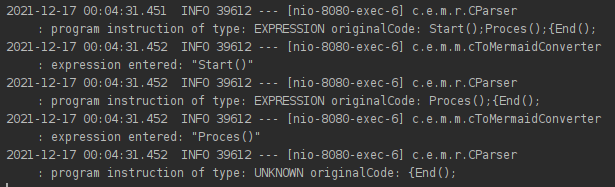
\includegraphics[width=\textwidth]{terminal-log.png}
  \end{subfigure}\hfill
  \caption{Przykładowy zapis w terminalu z przebiegu programu zakończonego błędem. }
\end{figure}
	

\section{Lexer i parser kodu języka C-podobnego}
	\subsection{Lexer} 
	W języku Java 11 SE stworzony został lexer kodu zintegrowany jest z parserem i jego podstawowym zadaniem jest rozpoznawanie instrukcji obsługiwanych przez aplikacje za pomocą wyrażeń regularnych oraz zapewnienia zrównoważonego użycia nawiasów zarówno okrągłych jak i klamrowych w odpowiedniej kolejności, zgodnie z zasadami programowania języka C. 

		\break
		
				
\begin{figure}[H]
  \begin{subfigure}{\textwidth}
			\begin{minted}[linenos=true]{java}
ELSE_PATTERN = "\\}else\\{.*";
IF_PATTERN = "if\\(.*";
WHILE_PATTERN = "while\\(.*";
EXPRESSION_PATTERN = "([\\w\\+\\-=\\(\\)\\.,<>/]+?;).*";
END_SCOPE_PATTERN = "\\}.*";
			\end{minted}
  \end{subfigure}\hfill
  \caption{Lista rozpoznawalnych przez lexer wyrazów regularnych (REGEX)}
\end{figure}
			
	\subsection{Parser} 		
	Parser kodu napisany jest w oparciu o recursive descent parser użyty m. in. w kompilatorach języka C takich jak: GCC oraz Clang. Polega on na rekursywnym wywoływaniu funkcji wczytującej kolejne instrukcje rozpoznane przez lexer oraz zależnie od rodzaju tych instrukcji wyciąga treść argumentu (w nawiasach okrągłych) oraz zawartość zakresu wewnętrznego (tzw. scope) instrukcji (w nawiasach klamrowych).		
						
\begin{figure}[H]
  \begin{subfigure}{\textwidth}
			\begin{minted}[linenos=true]{java}

private void handleIfStatement(){
    String statement = programBuilder.toString();
    String condition = getStringInOuterParenthesis(statement);
    String expressions = getStringInOuterCurly(statement);
    programBuilder.delete(0, condition.length() + 5);
    onIfStatementEnter(condition, expressions);
    parseProgramInstruction();
}
			\end{minted}
  \end{subfigure}\hfill
  \caption{Przykładowa funkcja, która izoluje z instrukcji $if$ jej argument (condition) oraz zawartość jej obszaru wewnętrznego (expressions), a następnie przekazuje te wartości do tzw. metody obserwowanej (onIfStatementEnter)}
\end{figure}
		
	 Otwarcie nowego zakresu w tym przypadku możliwe jest jedynie w instrukcjach $if - else$ oraz $while$. Aby umożliwić obsługę zagnieżdżeń tych instrukcji, enum reprezentujący jej typ z każdorazowym wejściem w jej zakres wewnętrzny (scope) jest odkładany na stos, a z wyjściem z zakresu zdejmowany z tego stosu co ma na celu późniejsze użycie samoczynnie wywołujących się metod obserwowanych (observable) we wzorcu projektowym $Obserwator$ ($Observer$). W przypadku instrukcji odpowiadającym procesom (dowolny tekst bez znaków specjalnych zakończony średnikiem) metoda obserwująca informuje jedynie o samym jej wywołaniu, natomiast w przypadku instrukcji warunkowych występują metody dedykowane wejściu oraz wyjściu z obszaru tej instrukcji. Domyślna metoda obserwowana jedynie wyświetla w terminalu podstawowe informacje o danej instrukcji, natomiast informacje te mogą być dowolnie wykorzystane wersji tej klasy z nadpisanymi definicjami jej metod obserwowanych. 
						
\begin{figure}[H]
  \begin{subfigure}{\textwidth}
		\begin{minted}[linenos=true]{java}
public void onIfStatementEnter(String condition, String expressions){
  log.info("IF entered : " + condition + " than : " + expressions);
}

public void onIfStatementExit(){
  log.info("IF exited");
}

public void onElseStatementEnter(String expressions){
  log.info("ELSE entered : " + expressions);
}
		\end{minted}
  \end{subfigure}\hfill
  \caption{Przykład domyślnych definicji metod obserwowanych dla instrukcji $if/else$}
\end{figure}



\section{Akcelerator budowania kodu w języku wymaganym przez Mermaid}

\begin{figure}[H]
  \begin{subfigure}{\textwidth}
  	\centering
    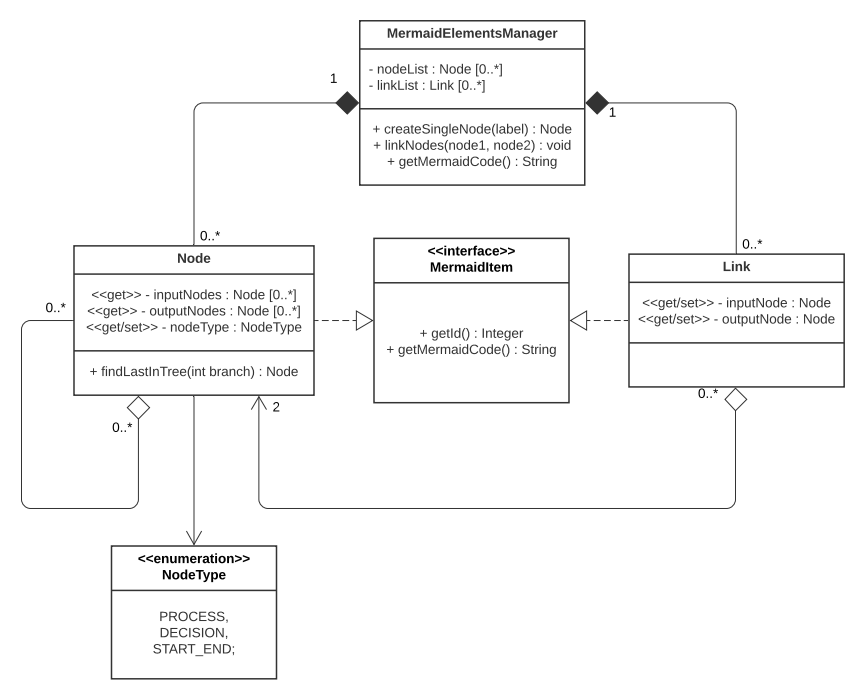
\includegraphics[width=\textwidth]{uml-akcelerator.png}
  \end{subfigure}\hfill
  \caption{Diagram UML klas z których powstał akcelerator budowania kodu Mermaid }
\end{figure}

	Do ułatwienia tworzenia schematów blokowych powstał akcelerator - zestaw klas, umożliwiający łatwe tworzenie i zarządzanie poszczególnymi elementami schematów blokowych, a następnie konwersja tych elementów w pamięci programu na kod docelowy, wymagany przez Mermaid. Docelowo składa się on z listy węzłów (nodes) odpowiadającym poszczególnym bloczkom oraz połączeniom (links) generowanym na podstawie relacji między tymi węzłami. 	Za pomocą akcesorów oraz innych publicznych metod wyszczególnionych na powyższym diagramie UML można w łatwy sposób tworzyć nowe węzły, nadawać im ich typ oraz łączyć je ze sobą.

\section{Konwerter kodu języka C-podobnego na język Mermaid}

	Konwerter ten wykorzystuje wcześniej wspomniany wzorzec projektowy Obserwator. W tym przypadku nadpisuje on domyślne definicje wcześniej opisanych metod obserwowanych. Zaraz po wywołaniu takiej nadpisanej metody, zależnie od tego do jakiej akcji została ona przypisana wykonuje określone akcje, również z argumentami przekazanymi przez te metody.
	
							
\begin{figure}[H]
  \begin{subfigure}{\textwidth}
		\begin{minted}[linenos=true]{java}
@Override
public void onIfStatementEnter(String condition, String expressions){
    condition = replaceChars(condition);
    condition = wordWrap(condition, 12);
    log.info("IF entered : " + condition + " than : " + expressions);
    manager.setLastNode(fromNode);
    NodeItem scopeNode = manager
            .createDecisionNodeLinkedToLast(condition);
    scopeNodes.push(scopeNode);
    fromNode = scopeNode.getOutputs().get(0);
}

@Override
public void onIfStatementExit(){
    log.info("IF exited");
    manager.createSingleNode("#if_merge");
    manager.linkNodes(scopeNodes.peek().findLastInTree(0), 
            manager.getLastNode());
    manager.linkNodes(scopeNodes.peek().findLastInTree(1), 
            manager.getLastNode());
    scopeNodes.pop();
    fromNode = manager.getLastNode();
}

@Override
public void onElseStatementEnter(String expressions){
    log.info("ELSE entered : " + expressions);
    fromNode = scopeNodes.peek().getOutputs().get(1);
}
		\end{minted}
  \end{subfigure}\hfill
  \caption{Przykład nadpisanych definicji metod obserwowanych dla instrukcji $if-else$}
\end{figure}

	Na powyższym przykładzie, po wejściu w instrukcję warunkową $if$ (onIfStatementEnter) warunek zostaje poddany usunięciu wszystkich specjalnych znaków, zastąpieniu znaku "\_" (underscore) przez " " (spacja). Następnie treść tego warunku poddana zostaje zawijaniu tekstu. Później po wstępnie przygotowanej zawartości warunku, z pomocą akceleratora budowania kodu Mermaid utworzony zostaje węzeł odpowiadający za bloczek decyzyjny. W związku z tym, że węzeł ten otwiera nowy obszar wewnętrzny (scope) zostaje on dodany do stosu (scopeNodes) śledzącego, który obszar jest w danym momencie wykonywany. Z bloczka decyzyjnego domyślnie wychodzą dwie gałęzi (jest połączony na wyjściu z dwoma pomocniczymi węzłami, które są niewidoczne), do końca pierwszej z nich (index = 0) przyłączane są kolejno instrukcje zawarte w obszarze wewnętrznym, odczytywane rekurencyjnie zgodnie z działaniem parsera, natomiast do końca drugiej gałęzi (index = 1) zostają przyłączane instrukcje po wywołaniu funkcji odpowiadającej instrukcji $else$. Po przetworzeniu całej zawartości opisywanej instrukcji warunkowej zostaje utworzony kolejny niewidoczny węzeł pomocniczy, który łączy obie gałęzie w momencie wychodzenia z obszaru wewnętrznego $if-else$ (wywołanie metody obserwowanej onIfStatementExit). Na koniec węzeł decyzyjny, którego obszar właśnie został zamknięty, zostaję zdjęty ze stosu.
	
	
	